\documentclass{article}


\include{stddefs}
\include{imodefs}

\newcommand{\vect}[2]{\begin{pmatrix} #1 \\ #2 \end{pmatrix}}
\newcommand{\vects}[3]{\begin{pmatrix} #1 \\ #2 \\ #3\end{pmatrix}}
\newcommand{\hphm}{\hphantom{-}}


\chapterno{5}

\begin{document}



\chapter{Euclidean vector spaces}

Big data are made up of many numbers in data sets. Such data sets can
be represented as vectors in a high dimensional euclidean vector
space. A vector is nothing but a list of numbers, but we need to talk
mathematically about the size of a vector and perform operations on
vectors. The term euclidean refers to vectors with a dot product as
known from the plane $\RR^2$.

The purpose of this chapter is to set the stage for this,
especially by introducing the dot product (or inner product) for
general vectors. Having a dot product is immensely useful and we give several
applications like linear regression and the perceptron learning algorithm

In the last part of the chapter rudimentary basics of analysis
are introduced like sequences, continuous functions, open, closed
and compact subsets. Some results will in this context only
be quoted and not proved.




\section{Vectors in the plane}

The dot product (or inner product) between two vectors $u, v\in \RR^2$ is
given by
\begin{equation}\label{smhack}
u\cdot v = x_1 x_2 + y_1 y_2,
\end{equation}
where
\begin{equation}
u = \begin{pmatrix} x_1 \\ y_1 \end{pmatrix}\qquad\text{and}\qquad
v = \begin{pmatrix} x_2 \\ y_2 \end{pmatrix}.
\end{equation}
We may also interpret
$u$ and $v$  as $2\times 1$ matrices (or column vectors).
Then the dot product in
\eqref{smhack} may be realized as the matrix product:
$$
u\cdot v = u^T v.
$$
The length or \emph{norm} of the vector $u\in \RR^2$ is given by
$$
\abs{u} = \sqrt{u\cdot u} = \sqrt{u^T u} = \sqrt{x_1^2 + y_1^2}.
$$
This follows from the \url{Pythagorean theorem}{https://en.wikipedia.org/wiki/Pythagorean_theorem}:

\includegraphics{Pythagoras.svg}


Also, the cosine of the angle $\theta$ between $u$ and $v$ is given by
$$
\cos(\theta) = \frac{u\cdot v}{\abs{u}\abs{v}}\qquad\text{or}\qquad u \cdot v = \abs{u} \abs{v} \cos(\theta).
$$
We will not go into this formula. It is a byproduct of considering the projection of a vector on
another vector (see Exercise \ref{dim2vec}).

\section{Higher dimensions}

The notions of dot product, norm and the formula for cosine of the
angle generalize immediately to vectors in dimensions
higher than two.

We denote the set of column vectors with $d$ rows
by $\RR^d$ and call it the euclidean vector space of
dimension $d$. An element $v\in \RR^d$ is called a vector and it has
the form (column vector with $d$ entries)
$$
v =
\begin{pmatrix}
  x_1 \\
  x_2 \\
  \vdots
  \\
  x_d
\end{pmatrix}.
$$

A vector in $\RR^d$ is a model for a data set in real life. A collection
of $d$ numbers, which could signify $d$ measurements. You will see
an example of this below, where a vector represents a data set
counting words in a string.

Being column vectors, vectors in $\RR^d$ can be added and multiplied by
numbers:
$$
\begin{pmatrix}
  x_1 \\
  x_2 \\
  \vdots
  \\
  x_d
\end{pmatrix} + 
\begin{pmatrix}
  y_1 \\
  y_2 \\
  \vdots
  \\
  y_d
\end{pmatrix}
=
\begin{pmatrix}
  x_1 + y_1 \\
  x_2 + y_2\\
  \vdots
  \\
  x_d + y_d
\end{pmatrix}\qquad\qquad
\lambda
\begin{pmatrix}
  x_1 \\
  x_2 \\
  \vdots
  \\
  x_d
\end{pmatrix} =
\begin{pmatrix}
  \lambda x_1 \\
  \lambda x_2 \\
  \vdots
  \\
  \lambda x_d
\end{pmatrix}.
$$

The dot product generalizes as follows to higher dimensions.

\subsection{Dot product and norm}

\begin{definition}[emph]
The dot product of
$$
u =
\begin{pmatrix}
  x_1 \\
  x_2 \\
  \vdots
  \\
  x_d
\end{pmatrix}\qquad
\text{and}
\qquad
v =
\begin{pmatrix}
  y_1 \\
  y_2 \\
  \vdots
  \\
  y_d
\end{pmatrix}
$$
is defined by
\begin{equation}\label{dotpr}
u\cdot v = u^T v = x_1 y_1 + x_2 y_2 + \cdots + x_d y_d.
\end{equation}


The norm of $u\in \RR^d$ is defined by
\begin{equation}\label{vecnorm}
\abs{u} = \sqrt{u\cdot u} = \sqrt{x_1^2 + x_2^2 + \cdots + x_d^2}.
\end{equation}


A vector $e\in \RR^d$ with $\abs{e}=1$ is called a \emph{unit vector}.

Two vectors $u, v\in \RR^d$ are called \emph{orthogonal} if $u\cdot v = 0$. We write
this as $u \perp v$.

\end{definition}

\beginshex
Show that
$$
u \perp u \iff u = 0,
$$
where $u\in \RR^d$.
\endshex


\beginshex\label{normrules}
Use the definition in \eqref{dotpr} to show that
\begin{align*}
  u\cdot (v + w) &= u\cdot v + u\cdot w\\
  (\lambda u)\cdot v &= u\cdot (\lambda v) = \lambda (u\cdot v)
\end{align*}
for $u, v, w\in \RR^d$ and $\lambda\in\RR$.
\endshex


\beginshex
Let $u\in \RR^d$ be a nonzero vector and $\lambda\in \RR$. Use the definition
in \eqref{vecnorm} to show that
$|\lambda u| = |\lambda| \, |u|$ and that
$$
\frac{1}{|u|} u
$$
is a unit vector.

\begin{hideinbutton}{Hint}
  You could perhaps use Exercise \ref{normrules} to do this. Notice also that
  $|\lambda|$ is the absolute value for $\lambda$ if $\lambda\in \RR$. 
\end{hideinbutton}
\endshex

\beginshex\label{dim2vec}
Given two vectors $u, v\in \RR^d$ with $v\neq 0$, find $\lambda\in \RR$, such
that $u - \lambda v$ and $v$ are orthogonal, i.e.
$$
(u - \lambda v) \cdot v = 0.
$$

\begin{hideinbutton}{Hint}
  $$
  (u - \lambda v) \cdot v = 0 \iff (u\cdot v) - \lambda (v\cdot v) = 0.
  $$
  This is an equation, where $\lambda$ is unknown!
\end{hideinbutton}

For $d=2$, it is sketched below
that if $u - \lambda v$ and $v$ are orthogonal, then
$u, \lambda v$ and $u-\lambda v$ are the sides in a right triangle.

\includegraphics{opggymkap5.png}


In this case, if $\theta$ is the angle between $u$ and $v$, show that
$$
\abs{u} \cos(\theta) = \abs{v} \lambda.
$$
Use this to show that
$$
u\cdot v = \abs{u} \abs{v} \cos(\theta).
$$
Finally show that
$$
\cos(A - B) = \cos(A) \cos(B) + \sin(A) \sin(B),
$$
where $A$ and $B$ are two angles.

\begin{hint}[showhide]
In the last question, you could use that the vectors
$$
\begin{pmatrix}
  \cos(A)\\ \sin(A)
\end{pmatrix}\qquad\text{and}\qquad
\begin{pmatrix}
  \cos(B)\\ \sin(B)
\end{pmatrix}
$$
are unit vectors.
\end{hint}
\endshex


\beginshex
Given two vectors $u, v\in \RR^d$, solve the minimization problem
\begin{align*}
  &\text{Minimize} &\abs{u - \lambda v}&\\
  &\text{with constraint}\\
  &&\lambda\in\RR.
\end{align*}

\begin{hint}[showhide]
  First convince yourself that $\lambda$ minimizes $\abs{u - \lambda v}$
  if and only if it minimizes
  $$
  (u - \lambda v)\cdot (u - \lambda v) = \abs{v}^2 \lambda^2 - 2 (u\cdot v)\lambda + \abs{u}^2,
  $$
  which happens to be a quadratic polynomial in $\lambda$.
\end{hint}
\endshex

\begin{quizexercise}[showhide]
\begin{quiz}
\question
Let $d$ denote the distance from $(1, 1)$ to the line through $(0, 0)$ and $(2, 1)$. What is true about $d$?
\answer{F}
$$
d = \frac{1}{2}.
$$
\answer{F}
$$
d = 0.447214.
$$
\answer{T}
$$
d = \frac{\sqrt{5}}{5}.
$$
\answer{F}
$$
d = \frac{2}{\sqrt{5}}.
$$
\end{quiz}
\end{quizexercise}



\begin{hideinbutton}{The dist formula from high school}
  The infamous \url{dist formula}{https://www.webmatematik.dk/lektioner/matematik-b/geometri/distanceformlen} from high school says that the distance from the point $(x_1, y_1)$ to the line
  given by $y = a x + b$ is
  \begin{equation}\label{distform}
  \frac{\abs{a x_1 + b - y_1}}{\sqrt{a^2 + 1}}.
  \end{equation}
  Where does this magical formula come from? Consider a general line $L$ in parametrized form
  $$
  L = \{ u + t v\mid t\in \RR\} \subseteq \RR^d.
  $$
  If $w\in \RR^d$, then the distance from $w$ to $L$ is given by the solution $t_0$ to the
  optimization problem
  \begin{align}\label{distopt}
  &\text{min}\, (w - (u + t v))\cdot (w - (u + t v))\\
  &t\in \RR.
\end{align}
This looks scary, but simply boils down to finding the top point of a parabola. The solution is
$$
t_0 = \frac{v\cdot w - u\cdot v}{v\cdot v}
$$
and the point on $L$ closest to $w$ is $u + t_0 v$.

Now we put
$$
u = \begin{pmatrix} 0 \\ b \end{pmatrix}, \quad v = \begin{pmatrix} 1 \\ a \end{pmatrix}\quad\text{and}\quad w = \begin{pmatrix} x_1 \\ y_1 \end{pmatrix}
$$
in order to derive \eqref{distform}. The solution to \eqref{distopt} becomes
$$
t_0 = \frac{x_1 + a y_1 - a b}{1 + a^2}.
$$
We must compute the distance $D$ from $w$ to $u + t_0 v$ in this case. The distance
squared is
\begin{align*}
D^2 &= |w - (u + t_0 v)|^2 = (w - (u + t_0 v))\cdot (w - (u + t_0 v)) \\ 
    &=(x_1 - t_0)^2 + (y_1 - b - t_0 a)^2.
\end{align*}
This is a mouthful and I have to admit that I used symbolic software (see below) to verify that
$$
D^2 = \frac{a^2 x_1^2 + 2 a b x_1 - 2 a x_1 y_1 + b^2 - 2 b y_1 + y_1^2}{1 + a^2} =
\frac{(a x_1 + b - y_1)^2}{1+a^2}.
$$
\begin{sage}
var('x1 y1 a b')
t0 = (x1 + a*y1 - a*b)/(1 + a^2)
D2 = (x1 - t0)^2 + (y1 - b - t0*a)^2
print(factor(D2))
\end{sage}
\end{hideinbutton}

\subsection{The perceptron algorithm}\label{sectperceptron}

Already at this point we have the necessary definitions for explaining the
perceptron algorithm. This is one of the early algorithms of machine learning.
It aims at finding a high dimensional line (hyperplane) that separates data
organized in two clusters.

In terms of the dot product, the core of the algorithm is described in
the example below.

\begin{example}\label{exampleperceptronsimple}




  Given finitely many vectors $v_1, \dots, v_n\in \RR^d$, can we find
  $\alpha\in \RR^d$, such that
  $$
  \alpha\cdot v_i > 0
  $$
  for every $i = 1, \dots, n$?


  
\beginshex
Come up with a simple example, where this problem is unsolvable i.e., come
up with vectors $v_1, \dots, v_n\in \RR^d$, where such an $\alpha$ does not
exist.

\begin{hideinbutton}{Hint}
  Try out some simple examples for $d=1$ and $d=2$.
\end{hideinbutton}  
\endshex

\beginshex
Suppose that there exists $\alpha\in \RR^d$, such that
$\alpha\cdot v_i > 0$ for every $i = 1, \dots, n$. Show then that
there exists $\alpha^*\in \RR^d$, such that
$$
\alpha^* \cdot v_i \geq 1
$$
for every $i = 1, \dots, n$.

\begin{hideinbutton}{Hint}
  Let $\mu = \min(\alpha\cdot v_1, \dots, \alpha\cdot v_n)$. Show that
  $\alpha^* = \frac{1}{\mu} \alpha$ works.
\end{hideinbutton}
\endshex

In case $\alpha$ exists, the following
ridiculously simple algorithm \footnote{works}{If you are interested in why the algorithm stops, click on the button after the example to read more about the perceptron algorithm} for finding $\alpha$:

  \begin{enumerate}[(i)]
  \item Begin by putting $\alpha = 0$.
  \item If there exists $v_i\in \{v_1, \dots, v_n\}$ with $\alpha\cdot v_i \leq 0$, then replace
    $\alpha$ by $\alpha + v_i$ and repeat this step. Otherwise $\alpha$ is the desired output vector.
  \end{enumerate}
    
Let us try out the algorithm on the simple example of just
two points in $\RR^2$ given by
$$
v_1 = \vect{-1}{\hphm 1}\qquad\text{and}\qquad v_2 =
\vect{1}{0}.
$$

In this case the algorithm proceeds as pictured below.



$$
\alpha = \vect{0}{0}\xrightarrow{+v_1} \vect{-1}{\hphm 1} \xrightarrow{+v_2} \vect{0}{1} \xrightarrow{+v_2}\vect{1}{1} \xrightarrow{+v_1}\vect{0}{2} \xrightarrow{+v_2} \vect{1}{2}.
$$

It patiently crawls its way ending with the vector $\alpha = \vect{1}{2}$, which
satisfies $\alpha\cdot v_1 > 0$ and $\alpha\cdot v_2 > 0$.

\includegraphics{perceptronsimple.png}

\end{example}


\begin{hideinbutton}{The perceptron algorithm}
The perceptron algorithm is a fancy name for a surprisingly simple
algorithm for computing a hyperplane that divides binary labeled
points.

We will assume that $x_1, \dots, x_n$ are
points in $\RR^d$ each of which is labeled by
a number $l_i\in \{-1, 1\}$.

Assuming that you can find a (separating) hyperplane $\alpha^T v = \beta$,
such that
$$
\alpha^T x_i > \beta\qquad\text{if}\qquad l_i = 1
$$
and
$$
\alpha^T x_i < \beta\qquad\text{if}\qquad l_i = -1.
$$


\includegraphics{perceptronsephyp.png}


We are interested in given the points and their labels in
computing $\alpha\in \RR^d$ and $\beta\in \RR$. In machine learning
the term \emph{training the algorithm} is used pointing
towards using the hyperplane for future points not in
the initial data set.


An extremely useful trick is to add one more dimension
and study the problem in $\RR^{d+1}.$ We replace
each point

$$
x_i\in \RR^d\qquad\text{ by }\qquad \hat{x_i} = (l_i x_i, l_i)\in \RR^{d+1}.
$$

The original problem is now equivalent to finding $\hat{\alpha}\in \RR^{d+1}\setminus\{0\}$,
such that
\begin{equation}\label{liftproblem}
\hat{\alpha}^T \hat{x_i} > 0
\end{equation}
for every $i = 1, \dots, n$. If such an $\hat{\alpha} = (\alpha_1, \dots, \alpha_d, t)^T$ can
be found, then we may take $\alpha = (\alpha_1, \dots, \alpha_d)^T$ and $\beta = -t$ as
a solution to our original problem.
On the other hand, if $\alpha$ and $\beta$ solve our original problem, then
$\hat{\alpha} = (\alpha, -\beta)$ solves \eqref{liftproblem}.


We have reduced our original problem to a simpler problem in
one more dimension. We will focus on this problem (now $d+1$ is
replaced by $d$):

Suppose that we are given points $x_1, \dots, x_n\in \RR^d$ and
there exists $\alpha\in \RR^d\setminus \{0\}$, such that
$\alpha^T x_i > 0$ for every $i = 1, \dots, n$. Geometrically
this means that all the points are on one side of the
hyperplane $\alpha^T v = 0$.

\includegraphics{perceptronsephpplusone.png}


We are interested in computing such an $\alpha$. This is exactly
what is done by the simple
algorithm presented in Example \ref{exampleperceptronsimple}.

\begin{example}\label{Examplepercep}
Consider the points
$$
v_1 = \vect{0}{0},\qquad v_2=\vect{1}{1}\qquad\text{and}\qquad v_3=\vect{\hphm 1}{-1}
$$
in $\RR^2$, where $v_1$ and $v_2$ are labeled by $+1$ and $v_3$ is labeled by $-1$. Then
$$
\hat{v}_1 = \vects{0}{0}{1},\qquad \hat{v}_2 = \vects{1}{1}{1}\qquad
\text{and}\qquad \hat{v}_3 = \vects{-1}{\hphm 1}{-1}.
$$
Now we run the simple algorithm from Example \ref{exampleperceptronsimple}:
$$
\hat{\alpha} = \vects{0}{0}{0}\xrightarrow{+\hat{v}_1} \vects{0}{0}{1} \xrightarrow{+\hat{v}_3} \vects{-1}{\hphm 1}{\hphm 0} \xrightarrow{+\hat{v}_1} \vects{-1}{\hphm 1}{\hphm 1}.
$$

From the last vector we see that $\alpha = \vect{-1}{\hphm 1}$ and $\beta = -1$ determine
a separating hyperplane (line) of the labeled points.

\includegraphics{perceptronplane.png}

\end{example}


\beginshex
Consider the points
$$
\begin{pmatrix}
0 \\ 0
\end{pmatrix},\qquad
\begin{pmatrix}
0 \\ 1
\end{pmatrix},\qquad

\begin{pmatrix}
1 \\ 1
\end{pmatrix},\qquad\text{and}\qquad
\begin{pmatrix}
1 \\ 0
\end{pmatrix}
$$
in $\RR^2$, where the first point is labeled with $-1$ and the rest by $1$.
Use the perceptron algorithm to compute a separating hyperplane.

What happens when you run the perceptron algorithm on the above
points, but where the label of
$$
\begin{pmatrix}
  1 \\ 1
\end{pmatrix}
$$
is changed from $1$ to $-1$?
\endshex


\begin{hideinbutton}{Why does the simple algorithm work?}
  We will assume that there exists $\alpha\in \RR^d$, such that
  $$
  \alpha^T x_i > 0
  $$
  for every $i = 1, \dots, n$. This is equivalent to the existence of $\alpha^*\in \RR^d$, such that
  $$
  (\alpha^*)^T x_i \geq 1
  $$
  for every $i = 1, \dots, n$. Let $r = \max\{\abs{x_1}, \dots, \abs{x_n}\}$. The basic insight
  is the following
  \begin{proposition}\label{proprepl}
    After $m$ replacements of $\alpha$ in the algorithm, we have
    \begin{align*}
      \alpha^T \alpha^* &\geq m \\
      m r^2 &\geq \abs{\alpha}^2.
    \end{align*}
  \end{proposition}
  \begin{proof}[showhide]
    These statements follow from the inequalities
    $$
    (\alpha + x_i)^T \alpha^* = \alpha^T \alpha^* + x_i^T \alpha^* \geq \alpha^T \alpha^* + 1
    $$
    and
    $$
    (\alpha + x_i)^T (\alpha + x_i) = \abs{\alpha}^2 + 2 x_i^T \alpha + \abs{x_i}^2 \leq \abs{\alpha}^2 +
    \abs{x_i}^2 \leq \abs{\alpha}^2 + r^2.
    $$
  \end{proof}

  Proposition \ref{proprepl} implies that
$$
m \leq \abs{\alpha} \abs{\alpha^*} \leq \sqrt{m} r \abs{\alpha^*}.
$$
Therefore we get $m\leq r^2 \abs{\alpha^*}^2$ and there is an upper bound on the number of
iterations used in the second step. At a certain iteration within this bound
we must have $\alpha^T x_i > 0$ for every $i=1, \dots, n$.
\end{hideinbutton}

Below is an implementation of the perceptron (learning) algorithm
in python with input from Example \ref{Examplepercep}.

\begin{sage}
import numpy as np

vectors = [[0,0], [1,1], [1,-1]]
labels = [1, 1, -1]

def liftvectors(vectors, labels):
    return [list(map(lambda t: x[1]*t, x[0]))+[x[1]] for x in zip(vectors, labels)]

def perceptron(inputvectors):
    alpha = np.array(len(inputvectors[0])*[0])
    vectors = list(map(np.array, inputvectors))
    done = False
    while not done:
        done = True
        for v in vectors:
            if np.dot(alpha, v) <= 0:
               alpha = np.add(alpha, v)  
               done = False
               break
    return alpha

print("The (normal) vector alpha in dimension one more is:")
    
perceptron(liftvectors(vectors, labels))    
\end{sage}

\beginshex
For python aficionados: why does the above code stop working when
\begin{quote}
  \texttt{vectors = list(map(np.array, inputvectors))}
\end{quote}
is replaced by
\begin{quote}
  \texttt{vectors = map(np.array, inputvectors)}
\end{quote}
?
\endshex

\end{hideinbutton}

\subsection{Bounded subsets}

A subset $S \subseteq \RR^d$ is called bounded if there exists $M\in \RR$, such that
$$
u\cdot u\leq M
$$
for every $u\in S$ i.e.,
\begin{frameit}
  $$
  u\in S \implies u\cdot u\leq M.
  $$
\end{frameit}

This condition is true if and only if there exists $N\in \RR$, such
that
$$
|u|\leq N
$$
for every $u\in S$ i.e., that the norms of the vectors in $S$ are bounded by some
number.

\beginshex
Describe geometrically what it means for a subset $S$ of $\RR$ resp. $\RR^2$
to be bounded by using intervals resp. circles (disks).
\endshex

\beginshex
Show precisely that the subset $\NN$ of $\RR$ is not bounded, whereas the subset
$\{1, \frac{1}{2}, \frac{1}{3}, \dots\}$ is.
\endshex

\beginshex
Sketch why
$$
S = \{(x, y) \mid x\geq 0, y\geq 0, x + y\leq 1\}\subseteq \RR^2
$$
is bounded. Now use Fourier-Motzkin elimination to show the same
without sketching.
\endshex

\subsection{Pythagoras and the least squares method}

The result below is a generalization of the theorem of Pythagoras about right
triangles to higher dimensions.

\begin{proposition}\label{proppythagoras}
  If $u, v\in \RR^d$ and $u\perp v$, then
  $$
  \abs{u + v}^2 = \abs{u}^2 + \abs{v}^2.
  $$
\end{proposition}

  \begin{proof}[showhide]
    This follows from
    $$
    (u + v)\cdot(u+v) = u\cdot u + u\cdot v + v\cdot u + v\cdot v = u\cdot u + v\cdot v = \abs{u}^2 + \abs{v}^2,
    $$
    since $u \cdot v = v\cdot u = 0$.
  \end{proof}




The dot product and the norm have a vast number of applications. One of them is the
method of least squares: suppose that you are presented with a system
\begin{equation}\label{lineqslsq}
A x = b
\end{equation}
of linear equations, where $A$ is an $m\times n$ matrix.

You may not be able to solve \eqref{lineqslsq}. There could be for example
$17$ equations and only $2$ unknowns making it impossible for all the equations to hold.
As an example, the system

\newcommand{\mph}{\phantom{-}}

\begin{equation}\label{nosols}
\begin{pmatrix}
\mph 1 & \mph 1\\
\mph 1 & -1\\
-1 & \mph 1
\end{pmatrix} \begin{pmatrix} x \\ y\end{pmatrix} = \begin{pmatrix} 3 \\ 1 \\ 1 \end{pmatrix}
\end{equation}
of three linear equations and two unknowns does not have any solutions.


The method of (linear) least squares seeks the best approximate solution $x_0$ to \eqref{lineqslsq} as a
solution to the minimization problem



\begin{align}\label{optlsq}
  &\text{Minimize} &\abs{b - A x}^2&\\
  &\text{with constraint}\\
  &&x\in\RR^n.
\end{align}

There is a surprising way of finding optimal solutions to \eqref{optlsq}:



\begin{theorem}[emph]\label{lsqthm}
  If $x_0\in\RR^n$ is a solution to the system
  $$
  (A^T A) x = A^T b
  $$
  of $n$ linear equations with $n$ unknowns,
  then $x_0$ is an optimal solution to \eqref{optlsq}.
\end{theorem}

  \begin{proof}[showhide]
    Suppose we know that $b - A x_0$ is orthogonal to $A v$ for every $v\in \RR^n$. Then
    $$
    \abs{b - A x}^2 = \abs{b - A x_0 + A(x_0 - x)}^2 = \abs{b - A x_0}^2 + \abs{A(x-x_0)}^2
    $$
    for every $x\in \RR^n$
    by Proposition \ref{proppythagoras}. So, in the case that
    $b - A x_0 \perp A v$ for every $v\in \RR^n$ we have
    $$
    \abs{b - A x}^2 \geq \abs{b - A x_0}^2
    $$
    for every $x\in \RR^n$ proving that $x_0$ is an optimal solution to
    \eqref{optlsq}.


    Now we wish to show that $b - A x_0$ is orthogonal to $A v$ for every $v\in \RR^n$ if and
    only if $A^T A x_0 = A^T b$. This is a computation involving the matrix arithmetic
    introduced in Chapter \ref{Chapter:Matrices}:
    \begin{align*}
      &(b - A x_0)\cdot A v = \\
      &(b - A x_0)^T A v  =\\
      &b^T A v - x_0^T A^T A v = \\
      &(b^T A - x_0 A^T A) v = 0
    \end{align*}
    for every $v\in \RR^n$ if and only if $b^T A - x_0 A^T A = 0$. But
    $$
    (b^T A - x_0 A^T A)^T = A^T b - A^T A x_0. 
    $$
  \end{proof}

In a future course on linear algebra you will see that the system of linear equations in
Theorem \ref{lsqthm} is always solvable i.e., an optimal solution to \eqref{optlsq} can
always be found in this way.



\beginshex
Show that \eqref{nosols} has no solutions. Compute the best approximate solution to \eqref{nosols} 
using Theorem \ref{lsqthm}.
\endshex

\begin{example}
  The classical application of the least squares method is to find
the best line $y = \alpha x + \beta$ through a given set of points
$$
(x_1, y_1), \quad (x_2, y_2), \quad \dots \quad, (x_n, y_n)
$$
in the plane $\RR^2$.

Usually we cannot find a line matching the points precisely. This corresponds to the fact that
the system of equations
$$
\begin{pmatrix}
x_1 & 1\\
x_2 & 1\\
\vdots & \vdots\\
x_n & 1
\end{pmatrix}
\begin{pmatrix}
\alpha \\ \beta
\end{pmatrix}
= 
\begin{pmatrix}
y_1 \\
y_2 \\
\vdots \\
y_n
\end{pmatrix}
$$
has no solutions.

Working with the least squares solution, we try to compute the best
line $y = \alpha x + \beta$ in the sense that
$$
(y_1 -\alpha x_1 -\beta)^2 + (y_2 -\alpha x_2 -\beta)^2 + \cdots +
(y_n -\alpha x_n -\beta)^2 
$$
is minimized.

\begin{figure}
\includegraphics{linreg.png}
\caption{Best fit of line to random points from \url{Wikipedia}{https://en.wikipedia.org/wiki/Least_squares}.}
\end{figure}

We might as well have asked for the best quadratic polynomial 
$$
y = \alpha x^2 + \beta x + \gamma 
$$
passing through the points
$$
(x_1, y_1), \quad (x_2, y_2), \quad \dots \quad, (x_n, y_n)
$$
in $\RR^2$.

The same method gives us the system
$$
\begin{pmatrix}
x_1^2 & x_1 & 1\\
x_2 ^2 & x_2 & 1\\
\vdots & \vdots\\
x_n^2 & x_n & 1
\end{pmatrix}
\begin{pmatrix}
\alpha \\ \beta \\ \gamma
\end{pmatrix}
= 
\begin{pmatrix}
y_1 \\
y_2 \\
\vdots \\
y_n
\end{pmatrix}
$$
of linear equations.


\begin{figure}
\includegraphics{parabelfit.png}
\caption{Best fit of quadratic polynomial to random points from  \url{Wikipedia}{https://en.wikipedia.org/wiki/Least_squares}.}
\end{figure}



The method generalizes naturally to finding the best polynomial of degree $m$
$$
y = a_m x^m + a_{m-1} x^{m-1} + \cdots + a_1 x + a_0 
$$
through a given set of points.
\end{example}

\beginshex
Find the best line $y = \alpha x + \beta$ through the points
$(1, 2), (2,1)$ and $(4,3)$ and the best quadratic polynomial
$ y = a x^2 + b x + c$ through the points
$(-2, 2), (-1, 1), (0,0), (1,1)$ and $(2,2)$.

It is important here, that you write down the relevant system
of linear equations according to Theorem \ref{lsqthm}.
It is however ok to solve the equations
on a computer (or check your best fit on \url{WolframAlpha}{https://www.wolframalpha.com/}).

Also, you can get a graphical illustration of your result in the sage window below.

\begin{sage}
pts = [(-2, 2), (-1, 1), (0, 0), (1, 1), (2, 2)]
a = 1
b = 1
c = 1
show(points(pts, pointsize=30) + plot(a*x^2 + b*x + c, (x, -2.5, 2.5)))
\end{sage}
\endshex


\beginshex
A circle with center $(a, b)$ and radius $r$ is given by the equation

\begin{equation}\label{eq:circle}
(x - a)^2 + (y - b)^2 = r^2.
\end{equation}

\begin{enumerate}
\item
  Explain how \eqref{eq:circle} can be rewritten to the equation
\begin{equation}\label{eq:circfit}
2 a x + 2 b y + c = x^2 + y^2,
\end{equation}
where $c = r^2 - a^2 - b^2$.

\item
  Explain how fitting a circle to the points $(x_1, y_1), \dots, (x_n, y_n)$
  in the least squares context using \eqref{eq:circfit} leads to the system
$$
\begin{pmatrix}
2 x_1 & 2 y_1 & 1\\
2 x_2 & 2 y_2 & 1\\
\vdots &\vdots &\vdots\\
2 x_n & 2 y_n & 1
\end{pmatrix}
\begin{pmatrix}
a \\
b \\
c
\end{pmatrix}
=
\begin{pmatrix}
x_1^2 + y_1^2\\
x_2^2 + y_2^2\\
\vdots \\
x_n^2 + y_n^2
\end{pmatrix},
$$
of linear equations.

\item

  Compute the best circle through the points
$$
(0, 2),\quad (0, 3),\quad  (2,0)\quad\text{and}\quad (3, 1)
$$ 
by giving the center coordinates and radius with two decimals.

\includegraphics{circlefit.png}

\end{enumerate}

\begin{sage}
pts = [(0, 2), (0, 3), (2, 0), (3, 1)]

x = 2
y = 2
r = 2

show(points(pts, pointsize=30) + circle((x, y), r))
\end{sage}

\endshex

\subsection{The Cauchy-Schwarz inequality}

Even though the generalizations of the dot product and norm to higher
dimensions amount to just adding some coordinates, they entail
a rather stunning result called the \url{Cauchy-Schwarz inequality}{https://en.wikipedia.org/wiki/Cauchy\%E2\%80\%93Schwarz_inequality}. The
proof is not long, but revolves around a rather beautiful trick.


\begin{theorem}\label{cs}
  For two vectors $u, v\in \RR^d$,
  $$
  \abs{u\cdot v} \leq \abs{u} \abs{v}.
  $$
\end{theorem}
  \begin{proof}[showhide]
    We consider the function $q:\RR\rightarrow \RR$ given by
    $$
    q(x) = (x u + v)\cdot (x u + v) = \abs{u}^2 x^2 + 2 (u\cdot v) x + \abs{v}^2
    $$
    Then $q(x)$ is a quadratic polynomial with $q(x)\geq 0$. Therefore
    its discriminant must be $\leq 0$ i.e.,
    $$
    4 (u\cdot v)^2 - 4 \abs{u}^2 \abs{v}^2 \leq 0,
    $$  
    which gives the result.
  \end{proof}


The Cauchy-Schwarz inequality
implies that 
$$
-1 \leq \frac{u\cdot v}{|u|\, |v|} \leq 1
$$
for two vectors $u, v\in \RR^d$ and it makes sense to define the angle
$\theta$ between these vectors\index{angle between vectors} by
\begin{equation}\label{cossim}
\cos(\theta) = 
\frac{u \cdot v}{|u|\, |v|}.
\end{equation}

\beginshex
For arbitrary two numbers $x, y\in \RR$, 
$$
2 (x^2 + y^2) \geq (x + y)^2,
$$
since
$$
2(x^2 + y^2) - (x + y)^2 = x^2 + y^2 - 2 x y = (x - y)^2\geq 0.
$$

Why is
$$
n (x_1^2 + \cdots + x_n^2) \geq (x_1 + \cdots + x_n)^2
$$
for arbitary $n$ numbers $x_1, \dots, x_n\in \RR$?
\endshex

\begin{example}

  When vectors are interpreted as data sets,
  the number in \eqref{cossim} is known as the \emph{cosine similarity}
and measures the correlation between the two data sets
$u$ and $v$.

An application could be the similarity between two strings.
Consider the two strings 
"\emph{Mathematics is fun and matrices are useful}"
and
"\emph{Mathematics is fun and matrices are applicable}".

From the words in the two strings we form the following vectors in $\RR^8$.

$$
\begin{array}{lll}
  \text{Mathematics} & 1 & 1\\[0.5em]
  \text{is} & 1& 1\\[0.5em]
  \text{fun} & 1 & 1\\[0.5em]
  \text{and} & 1 & 1\\[0.5em]
  \text{matrices} & 1 & 1\\[0.5em]
  \text{applicable} & 0 & 1\\[0.5em]
  \text{useful} & 1 & 0\\[0.5em]
  \text{are} & 1 & 1
\end{array}
$$

where every word in the two strings has an entry counting the number of
occurences in the string. A measure for the equality between
the two strings is the cosine of the angle between the two vectors.

The closer the cosine gets to $1$ (corresponding to an angle of $0$
degrees), the more similar we consider the strings.

In the above case the cosine similarity is approximately $0.86$.

Below is a snippet of python code (using \texttt{numpy}) for computing the cosine similarity of two strings, where
words are separated by blanks. It can be extended in many ways.


\begin{sage}
import numpy as np
from numpy.linalg import norm

def cosinesim(str1, str2):
  words1 = str1.split()
  words2 = str2.split()
  words12 = list(set().union(words1, words2))
  v1 = np.array([words1.count(w) for w in words12])
  v2 = np.array([words2.count(w) for w in words12])
  return (np.dot(v1, v2)/(norm(v1)*norm(v2)))

str1 = "Mathematics is fun and matrices are useful"
str2 = "Mathematics is fun and matrices are applicable"

print("The cosine similarity between")
print(str1)
print("and")
print(str2)
print("is")
print(cosinesim(str1, str2))
\end{sage}


This application is based on rather basic mathematics, but we do get a quantitative measure for
how close two strings are. This is a crude tool applicable for flagging potential plagiarism.

The cosine similarity is implemented in the python machine
learning library \url{\texttt{sci-kit-learn}}{https://scikit-learn.org/stable/}.

\end{example}



\subsection{Distance of vectors and the triangle inequality}

We know how to measure the size of a vector $u\in \RR^d$ by its norm $\abs{u}$. We need
to measure how close two vectors $u, v\in \RR^d$ are i.e., we
need to measure their \emph{distance}. A perfectly good
measure for the distance from $u$ to $v$ is the norm
$$
\abs{u-v}.
$$
You can see from \eqref{vecnorm} that $|u-v|$ is small implies that
the coordinates of $u$ and $v$ are close. Also we want $u = v$ if
their distance is zero. This is satisfied. Similarly we want
the distance from $u$ to $v$ to equal the distance from $v$ to $u$. This is true,
since $\abs{x} = \abs{-x}$ for any vector $x\in \RR^d$.

\beginshex
Show the above, that $\abs{x} = \abs{-x}$ for any vector $x\in \RR^d$. Explain why
this implies $\abs{u - v} = \abs{v - u}$ for every $u, v\in \RR^d$.
\endshex

One other, not so obvious property, is the \url{triangle inequality}{https://en.wikipedia.org/wiki/Triangle_inequality}.

\begin{theorem}\label{thmtrineq}
  For two vectors $u, v\in \RR^d$,
  $$
  \abs{u + v} \leq \abs{u} + \abs{v}.
  $$
  \end{theorem}
    \begin{proof}[showhide]
      From the Cauchy-Schwarz inequality (Theorem \ref{cs}) it follows that 
      $$
      \abs{u+v}^2 = (u+v)\cdot (u+v) = \abs{u}^2 + 2 u\cdot v + \abs{v}^2 \leq \abs{u}^2 + 2 \abs{u}\abs{v} + \abs{v}^2.
      $$
      Since the right hand side of this inequality is $(\abs{u} + \abs{v})^2$, the result follows.
    \end{proof}

  Why is this result called the triangle inequality? A consequence is that
  $$
  \abs{u - v}  = \abs{(u - w) + (w - v)} \leq \abs{u - w} + \abs{w - v},
  $$
  i.e., that the distance from $u$ to $v$ is always less than or equal to
  the distance from $u$ to $w$ plus the distance from $w$ to $v$, where
  $w$ is a third vector.

  In boiled down terms: the length of any one side in a triangle is
  less than or equal to the sum of the lengths of the two other sides.


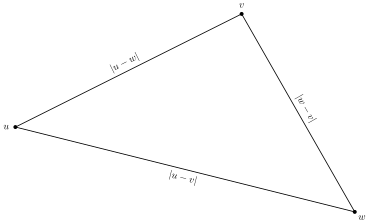
\includegraphics{triangleineq.svg}

\beginshex
Find two typos in the figure above. Correct them!
\endshex

The triangle inequality implies that
\begin{align}\label{trineqopp}
  \abs{\abs{x}-\abs{y}} &\leq \abs{x - y}\\
  \abs{\abs{x}-\abs{y}} &\leq \abs{x + y}
\end{align}
for every $x, y\in \RR^d$.

\beginshex
  Show how \eqref{trineqopp} follows from Theorem \ref{thmtrineq}. 
\endshex




\section{An important remark about the real numbers}

In the beginning of this course, we postulated the existence of the real
numbers $\RR$ as an extension of the rational numbers $\QQ$ with their ordering $\leq$.

The rational numbers had the glaring defect that the graph of the function $f:\QQ\rightarrow \QQ$ given by
$$
f(x) = x^2 - 2
$$
does not intersect the $x$-axis between $1$ and $2$ in spite of the
fact that $f(1) = -1$ and $f(2) = 2$.


It seems from the sage plot below, that the graph intersects the
$x$-axis around $x_0\approx 1.4$, but it really does not happen!
Your computer and its screen only
handles rational numbers.

\begin{sage}
  plot(x**2 -2, (x, 1, 2))
\end{sage}

Surely the most natural property for a well behaved function
(like $f(x) = x^2 - 2$) is that it must intersect the $x$-axis
in a point $x_0$ with $a < x_0 < b$ if $f(a) < 0$ and $f(b) > 0$.

I will not be completely precise about how to repair this defect about the
rational numbers $\QQ$, but
just state one exceedingly important property about the real numbers $\RR$ in
the button below.

In fact this
one property guarantees that $\RR$ does not have any holes
as in the graph above.


\begin{hideinbutton}{Supremum and infimum}
\subsection{Supremum}

A subset $S$ of $\RR$ is called \emph{bounded from above} if there exists
$M\in \RR$, such that $x\leq M$ for every $x\in S$. Here $M$ is
called an \emph{upper bound} for $S$.

\beginshex
Give an example of a subset of the real numbers, which is not bounded from
above and one that is.
\endshex


The set of real numbers satisfies that for every subset $S\subseteq \RR$ bounded from above,
 there exists a smallest upper bound denoted $\sup(S)$ called
the \emph{supremum} of $S$. In precise terms,
\begin{enumerate}[(i)]
\item
  $\sup(S)\geq x$ for every $x\in S$ 
\item
  If we move a little to the left of $\sup(S)$ we encounter
  elements from $S$: for every $\epsilon > 0$, there exists $x\in S$,
  such that
  $$
  \sup(S)-\epsilon < x \leq \sup(S).
  $$
\end{enumerate}

\includegraphics{supremum.png}

Notice that we may have $\sup(S)\not\in S$.

\subsection{Infimum}

In the same way a subset $S$ of $\RR$ is called \emph{bounded from below}, if
there exists $m\in \RR$, such that $m \leq x$ for
every $x\in S$. Every subset $S$ bounded from below has
a largest lower bound denoted $\inf(S)$ called the \emph{infimum} of $S$.
In precise terms,
\begin{enumerate}[(i)]
\item
  $\inf(S)\leq x$ for every $x\in S$ 
\item
  If we move a little to the right of $\inf(S)$ we encounter
  elements from $S$: for every $\epsilon > 0$, there exists $x\in S$,
  such that
  $$
  \inf(S) \leq x < \inf(S) + \epsilon.
  $$
\end{enumerate}


\beginshex
Give a simple example of a subset $S\subseteq \RR$ bounded from above, where
$\sup(S)\not\in S$.

Show that the subset $S = \{x\in \QQ \mid x^2 < 2\}$ of $\RR$ is bounded from above and below and
  that $\sup(S)\not\in \QQ$ and $\inf(S)\not\in \QQ$.
\endshex

\beginshex
Show that $S$ is infinite if $\sup(S)\not\in S$.
\endshex

\end{hideinbutton}



  \section{Sequences and limits in $\RR^d$}

  For the first time in the notes we are now moving towards infinite
  processes. We will introduce limits
  of vectors organized in an infinite sequence.

\begin{definition}[emph]  
A sequence
in  $\RR^d$ is an \emph{infinite} list of vectors
$$
v_1, v_2, v_3, \dots
$$
in $\RR^d$, where repetitions are allowed. Such a sequence is denoted $(v_n)$.
\end{definition}

In order to define a sequence we just need to tell what its $n$-th element is. So
in abstract terms a sequence in $\RR^d$ is nothing but a function $\NN\rightarrow \RR^d$.

\begin{example}
Below we give two examples of sequences in $\RR$.
\begin{align*}
&(x_n): 1, 2, 3, 4, \dots\\
&(y_n): 1, \tfrac{1}{2}, \tfrac{1}{3}, \tfrac{1}{4}, \dots
\end{align*}
The first sequence is given by $x_n = n$ and the second $y_n = \frac{1}{n}$ for $n\in \NN$. The first sequence
explodes to infinity, whereas the second sequence gets closer and closer to $0$. In the latter case we
write
$$
\lim_{n\to\infty} y_n = 0.
$$
\end{example}

What does it mean that a sequence $(v_n)$ of vectors in $\RR^d$  has limit $v\in \RR^d$? Intuitively,
we can get $v_n$ as close to $v$ as we want by choosing
$n\in \NN$ sufficiently big. Here is the precise way of saying this:


\begin{equation}[emph]\label{convdef}
\forall \epsilon > 0\, \exists N\in \NN: n\geq N\implies \abs{v_n - v} < \epsilon.
\end{equation}


If a sequence $(v_n)$ has a limit $v$, then we write
$$
\lim_{n\to\infty} v_n = v.
$$

A sequence is called convergent if it has a limit. Let us see
how our new technology works on two intuitively
obvious examples.





\begin{example}\label{Example:basicconv}
  Let us use \eqref{convdef} to give a precise proof of
  $$
  \lim_{n\to\infty} x_n = 0,
  $$
  where $x_n = 1/n$. So given any $\epsilon >0$ we must find $N\in \NN$, such that
  $$
  \abs{x_n - 0} = \abs{x_n} = \frac{1}{n} < \epsilon
  $$
  for $n > N$. But
  $$
  \frac{1}{n} < \epsilon \iff \frac{1}{\epsilon} < n.
  $$
  So we simply choose $N$ to be the smallest natural number bigger than $\frac{1}{\epsilon}$.

  An even simpler example is a constant sequence like
  $$
  17, 17, 17, 17, \dots
  $$
  i.e., $x_n = 17$ for all $n\in \NN$. Here we want the limit to be $17$ and
  \eqref{convdef} agrees. We can put $N= 1$:
  $$
  \forall \epsilon > 0 : n\geq 1\implies \abs{x_n - 17} = \abs{17 - 17} = 0 < \epsilon.
  $$

\end{example}


If a sequence is convergent, then it can have
only one limit. You can not have a convergent sequence with two different limits!
In particular, the constant sequence
$$
  17, 17, 17, 17, \dots
  $$
  cannot converge to $18$.

\beginshex
Give a precise proof of the fact that a convergent sequence $(x_n)$ can only have
one limit using proof by contradiction i.e., start by assuming that
it has two different limits $x\neq y$. Then show that 
$$
\forall \epsilon > 0\, \exists N\in \NN: n\geq N\implies \abs{x_n - y} < \epsilon.
$$
cannot be true by showing that
$$
\exists \epsilon > 0\, \forall N\in \NN: \exists n\geq N\implies \abs{x_n - y} \geq \epsilon.
$$
\begin{hint}
  Try $\epsilon = \abs{x-y}/2$ in the definition of $x$ being a limit and apply \eqref{trineqopp} to
  $$
  \abs{x_n - y} = \abs{x_n - x + x - y}.
  $$
\end{hint}
\endshex

Now, that we have the definition of a convergent sequence, we go on to use it in a rather
typical proof of a rather typical result. In this (typical) proof we first handle the
infinite and then the finite.




\begin{proposition}\label{propconvbounded}
  A convergent sequence $(x_n)$ is bounded i.e., there exists $M\in \RR$, such that
  $|x_n| \leq M$ for every $n\in \NN$.
\end{proposition}
  \begin{proof}[showhide]
    Let $x$ denote the limit of $(x_n)$. Then for $\epsilon = 1$, we may find
    $N\in \NN$, such that $\abs{x - x_n} < 1$ for $n\geq N$. Therefore
    $\abs{x_n} < \abs{x} + 1$ for $n\geq N$ by \eqref{trineqopp}. Let
    $M_1 = \max\{\abs{x_0}, \dots, \abs{x_N}\}$ and then letting
    $M = \max\{M_1, \abs{x} + 1\}$, we see that $\abs{x_n} \leq M$
    for every $n\in \NN$.
  \end{proof}


  \begin{example}
    Proposition \ref{propconvbounded} shows that the sequence
    $$
    1, 2, 3, 4, \dots
    $$
    cannot be convergent. Why?
  \end{example}


  


\newcommand{\phmi}{\phantom{-}}
\begin{quizexercise}[showhide]
\begin{quiz}
  \question
  What is the limit of the sequence
  $$
  \phmi 1, -1, \phmi 1, -1, \phmi 1, -1, \dots ?
  $$
  \answer{F}
  $$1$$
  \answer{F}
  $$-1$$
  \answer{T}
  It does not have a limit.
  \answer{F}
  $$0$$
\end{quiz}
\end{quizexercise}

Sage may be helpful in computing limits (see below).

\begin{sage}
n = var('n')
assume(n>0)
sequence = n/(n+1)
limit(sequence, n=infinity)
\end{sage}


For convergent sequences we have the following result.

\begin{frameit}
\begin{proposition}\label{propconvarithm}
Let $(x_n)$ and $(y_n)$ be convergent sequences in $\RR^d$ with limits
$x$ and $y$ respectively. Then
\begin{enumerate}[(i)]
\item\label{itemsum}
the sequence $(x_n + y_n)$ is convergent with limit $x + y$.
\item\label{itemproduct}
the sequence $(x_n y_n)$ is convergent with limit $x y$ (if $d=1$)
\item
the sequence $(x_n/y_n)$ is convergent with limit $x/y$ provided
that $y\neq 0$ and $y_n \neq 0$ for every $n\in\NN$ (if $d=1$).
\end{enumerate}
\end{proposition}
\end{frameit}
  \begin{proof}[showhide]
    I will give the proof of \ref{itemproduct}. By definition (see
    \eqref{convdef}) we are given $\epsilon > 0$ and we must find
    $N\in \NN$, such that
    $$
    \abs{x y - x_n y_n} < \epsilon
    $$
    for $n\geq N$. An old trick shows that
    $$
    \abs{x y - x_n y_n} = \abs{(x-x_n) y + (y - y_n) x_n}.
    $$
    Therefore we may find $M > 0$ so that 
    $$
    \abs{x y - x_n y_n} \leq \abs{x-x_n}\abs{y} + \abs{y - y_n}\abs{ x_n} \leq \abs{x-x_n} M + \abs{y-y_n} M,
    $$
    where $y \leq M$ and $\abs{x_n}\leq M$ for every $n\in \NN$ (see Proposition \ref{propconvbounded}).
    We are assuming the $(x_n)$ and $(y_n)$ are convergent sequences. Therefore we may find
    $N_1$ and $N_2$ in $\NN$, so that
    \begin{align*}
      \abs{x - x_n} &< \frac{\epsilon}{2 M}\qquad\text{for}\qquad n \geq N_1\\
      \abs{y - y_n} &< \frac{\epsilon}{2 M}\qquad\text{for}\qquad n \geq N_2.
    \end{align*}
    Choosing $N = \max\{N_1, N_2\}$, we get
    $$
    \abs{x y - x_n y_n} \leq \abs{x-x_n} M + \abs{y-y_n} M \leq \frac{\epsilon}{2 M} M + \frac{\epsilon}{2 M} M = \epsilon,
    $$
    for $n\geq N$.
  \end{proof}

\beginshex
The proof of \ref{itemsum} in Proposition \ref{propconvarithm} is much less involved
than the given proof of \ref{itemproduct} in the same result. In the proof of
\ref{itemproduct} we used a trick using $\frac{\epsilon}{2M}$. Use the same
trick with $\frac{\epsilon}{2}$ and the triangle inequality to prove
\ref{itemsum}.
\begin{hint}
  $$
  \abs{x + y - (x_n + y_n)} = \abs{(x - x_n) + (y - y_n)} \leq \abs{x - x_n} + \abs{y - y_n}. 
  $$
\end{hint}
\endshex

\begin{quizexercise}[showhide]
  \begin{quiz}
    \question
    What is the limit of the sequence $(x_n)$ given by
    $$
    x_n = \frac{3 n^2 + 17 n + 5}{2 n^2 + 3 n + 2}?
    $$
    \answer{F}
    $$0$$
    \answer{F}
    It does not have a limit
    \answer{T}
    $$1.5$$
    \answer{F}
    $$\frac{17}{5}$$
  \end{quiz}
\end{quizexercise}


\beginshex
Consider the sequence $(x_n)$ given by
$$
x_n = \left(1 + \frac{1}{n}\right)^n.
$$
Carry out a computer experiment in Sage below to find the limit
of $(x_n)$. Can you prove what you observe in
the experiment?

\begin{sage}
def exp(n):
  print("(1 + 1/n)^n is =")
  print((1 + 1/float(n))**n)
  print("for n = ", n)

exp(100)  
\end{sage}

\begin{hint}
  $$
  n \ln\left(1 + \frac{1}{n}\right) =
  \frac{\ln\left(1 + \frac{1}{n}\right) - \ln(1)}{\frac{1}{n}}
$$
\end{hint}
\endshex

\beginshex
Assume that $(x_n)$ is a convergent sequence in $\RR^d$. Show that
$(\abs{x_n})$ is a convergent sequence in $\RR$.
\endshex

\beginshex
Let $(x_n)$ be a sequence bounded below with the property that
$$
x_1 \geq x_2 \geq x_3 \geq \cdots
$$
Show that $\inf\{x_n \mid n\in \NN\}$ is the limit of $(x_n)$.

Similarly let $(z_n)$ be a sequence bounded above with the property that
$$
z_1 \leq z_2 \leq z_3 \leq \cdots
$$
Show that $\sup\{z_n \mid n\in \NN\}$ is the limit of $(z_n)$.
\endshex

\beginshex
\begin{enumerate}[(i)]
\item Show that
  $$
  \sqrt{a b} \leq \frac{a+b}{2},
  $$
  for $0 \leq a \leq b$.
\item
  Prove that $a < \sqrt{a b}$ and $(a+b)/2 < b$ for $0\leq a < b$.
\item
  Start with two numbers $a$ and $b$ with $0\leq a\leq b$ and define
  \begin{align*}
    a_{n+1} &= \sqrt{a_n b_n}\\
    b_ {n+1} &= (a_n + b_n)/2,
  \end{align*}
  where $a_0 = a$ and $b_0 = b$. Carry out computer experiments in the sage (python) window below
  to analyze the sequences $a_0, a_1, \dots$ and $b_0, b_1, \dots$
  for different values of $a_0$ and $b_0$.


\begin{sage}
import math

a0 = 1
b0 = 2
print("Input a=", a0, " and b=", b0)
print("Iterating towards ag mean:")
  
for i in range(10):
  print(a0, b0)
  a1 = math.sqrt(a0*b0)
  b1 = (a0 + b0)/float(2)
  a0 = a1
  b0 = b1
\end{sage}
\item
  Prove for $n\geq 1$ that
  $$
  b_n - a_n < \left(\frac{1}{2}\right)^n (b-a)
  $$
  if $0< a < b$.
\item
  Let $s = \lim_{n\to \infty} a_n$ and $t=\lim_{n\to \infty} b_n$.
  Show that the limits exist and that $s = t$.
\end{enumerate}
The common limit $M(a, b)$ of the sequences $(a_n)$ and
$(b_n)$ is called the \url{arithmetic-geometric mean}{https://en.wikipedia.org/wiki/Arithmetic\%E2\%80\%93geometric_mean} of $a$ and $b$.
Just for the fun of it, here is a cool way of computing $\pi$
involving this quantity:
$$
\pi = \frac{4 M(1, \frac{1}{\sqrt{2}})^2}{1 - \sum_{n=1}^\infty 2^ {n+1}(b_n^2 - a_n^2)}.
$$
\endshex

\subsection{Closed and open subsets}

We have defined what it means for a subset of a euclidean space to be bounded. Now
we come to an exceedingly important definition about subsets being closed meaning
that they should (in a mathematically precise way) contain their boundary points. For example, we want the interval $[0, 1]$ to be closed, whereas the
interval $[0, 1)$ should not be closed, because it is missing its
boundary point $1$.

\begin{definition}[emph]
A subset $F\subseteq \RR^d$ is called closed if it contains all its limit vectors. This
means that if $(v_n)$ is a convergent sequence contained in $F$, then its limit must
be contained in $F$.
\end{definition}




We can immediately come up with a non-closed subset using the definition. Consider the subset
$$
S = \{x\in \RR \mid x > 0\}\subset \RR.
$$
Here $\left(\frac{1}{n}\right)$ is a convergent sequence, whose elements all are
contained in $S$, but its limit $0$ is outside $S$ (see Example
\ref{Example:basicconv}).
We have, however, the following important result relating to this example.

\begin{proposition}[emph]\label{closedinR}
  The following subsets
  \begin{align*}
    [a, b] &= \{x\in \RR \mid a \leq x \leq b\} \\
    [a, \infty) &= \{x\in \RR \mid a \leq x\}\\
    (-\infty, a] &= \{x\in \RR \mid x \leq a\}
  \end{align*}
  are closed subsets of $\RR$ for every $a, b\in \RR$.
\end{proposition}

Closed subsets are preserved by finite unions and intersections.

\begin{proposition}[emph]
  Let $F_1, F_2, \dots, F_n$ be finitely many closed subsets of $\RR^d$. Then 
  $$
  F_1 \cap F_2 \cap \cdots \cap F_n \qquad\text{and}\qquad
  F_1 \cup F_2 \cup \cdots \cup F_n 
  $$
  are closed subsets of $\RR^d$.
\end{proposition}

The complementary notion of a closed subset is an open subset.


\begin{definition}[emph]
  A subset $U\subseteq \RR^d$ is called \emph{open} if $\RR^d\setminus U$ is closed.
\end{definition}

\beginshex
Prove that 
  $$
  U_1 \cap U_2 \cap \cdots \cap U_n \qquad\text{and}\qquad
  U_1 \cup U_2 \cup \cdots \cup U_n 
  $$
if $U_1, \dots, U_n$ are open subsets.
\endshex

  \beginshex
  Let $(a, b) =\{x \in \RR \mid a < x < b\}$ for $a, b\in \RR$, where $a < b$.
  Show that $(a, b)$ is an open subset of $\RR$.
  \endshex

  \begin{remark}
    In fact, an arbitrary (also infinite) intersection of closed subsets is closed and an arbitrary (also infinite) union of open subsets is open. However, for a
    first course introducing intersections and unions over arbitrary families is pushing the
    envelope.
  \end{remark}
  

\begin{hideinbutton}{Infinite series}
\subsection{Infinite series}

Given a sequence $(x_m)$ in $\RR^d$ we may form the new sequence given by the sums
\begin{align*}
  s_1 &= x_1\\
  s_2 &= x_1 + x_2\\
      &\vdots\\
  s_n &= x_1 + x_2 + \cdots + x_n\\
  &\vdots       
\end{align*}
Such a sequence is called an infinite series. It is denoted
$$
\sum_{n=1}^\infty x_n
$$
and is defined to converge if the sequence $(s_n)$ converges.

Infinite series give rise to very \url{beautiful identities}{https://en.wikipedia.org/wiki/Basel_problem} like
$$
\sum_{n=1}^\infty \frac{1}{n^2} = \frac{\pi^2}{6}.
$$

We will not go deeper into the rich theory of infinite series, but
settle at defining a widely used infinite series called the
\emph{geometric series}.  Let $q\in \RR$ with $\abs{q} < 1$. We saw in
the first chapter that
$$
1 + q + \cdots + q^n = \frac{1 - q^{n+1}}{1-q}
$$
for any number $q\neq 1$. If $\abs{q} < 1$, then $\lim_{n\to\infty} q^n = 0$.

\beginshex
Show that $\lim_{n\to\infty} q^n = 0$ if $\abs{q} < 1$.
\endshex

Therefore
\begin{equation}\label{geomseries}
  \sum_{n=0}^\infty q^n = \frac{1}{1-q}.
\end{equation}
The series in \eqref{geomseries} is called the geometric series.

\beginshex
Compute the (infinite) sums
\begin{enumerate}[(i)]
\item
  $$
  \frac{1}{2} + \frac{1}{4} + \frac{1}{8} + \cdots
  $$
\item
  $$
  1 - \frac{1}{2} + \frac{1}{4} - \frac{1}{8} + \cdots
  $$
\end{enumerate}
\endshex

\beginshex
The series given by $x_n = \frac{1}{n}$ i.e.,
$$
s_n = 1 + \frac{1}{2} + \frac{1}{3} + \cdots + \frac{1}{n}
$$
is called the \emph{harmonic series}. Explore the growth of the harmonic series as a function of $n$
using the sage window below.

\begin{sage}
n = 100
print("The sum of the first ", n , " terms in the harmonic series is ", sum(1/float(i) for i in range(1, n+1)))
\end{sage}

What does this \url{video}{https://twitter.com/TamasGorbe/status/1174406602998341632/video/1}
on twitter have to do with the harmonic series?

Suppose that the inequality
\begin{align}\label{lbharm}
\ln(n) = \int_1^n \frac{1}{x} d x \leq 1 + \frac{1}{2} + \cdots + \frac{1}{n}
\end{align}
holds. What does \eqref{lbharm} imply for the harmonic series? Is \eqref{lbharm} true? Compare
with the graphs in the sage window below.

\begin{sage}
n = 1000
  
print("Graphs of the sum of the harmonic series and the (natural) logarithm (red) up to n=", n)
x = var('x')
g = Graphics()
g += plot(harmonic_number(x), (x, 1, n))
g += plot(log(x), (x, 1, n), color='red')
g.show()
\end{sage}

Use the sage window below to investigate if the sequence $e_n$ given by
$$
e(n) = 1 + \frac{1}{2} + \cdots + \frac{1}{n} - \ln(n)
$$
converges. In particular, make a clever statement about the convergence by studying a finite table
of
$$
e(1), e(2), e(3), \dots
$$
observing $e(n) - e(n+1)$ for $n = 1, 2, 3, \dots$.

\begin{sage}
def euler(n):
  return harmonic_number(float(n)) - log(float(n))

n = 100
print("e(n) is ", euler(n), " for n=", n )
\end{sage}
\endshex


\end{hideinbutton}


\section{Continuous functions}

\begin{definition}[emph]\label{defcontfunc}
A function $f: S\rightarrow T$, where $S \subseteq \RR^d$ and $T\subseteq \RR^e$ is
called \emph{continuous at $v\in S$} if for every
convergent sequence $(v_n)$ in $S$ with limit $v\in S$, $(f(v_n))$ is a
convergent sequence with limit $f(v)$ in $T$. The function $f: S\rightarrow T$ is called continuous
if it is continuous at every $v\in S$.
\end{definition}


The above is the formal definition of a continuous function. It is short and sweet. To
get an understanding, you should study the mother of all examples of 
non-continuous functions given below:
\begin{equation}\label{bracketfct}
f(x) =
\begin{cases}
  0 &\text{if } x > 0\\
  1 &\text{if } x \leq 0
\end{cases}.
\end{equation}

This is a function from $\RR$ to $\RR$. It is impossible to plot it
without lifting the pencil or defining such a beast without using a
bracket as in \eqref{bracketfct}.

\includegraphics{noncont.png}

Let me sketch how the formal Definition \ref{defcontfunc} kills any hope of
\eqref{bracketfct} being continuous. It is enough to come up with just
one sequence $(x_n)$ converging to $x$, such that the sequence
$(f(x_n))$ does not converge to $f(x)$.  We pick
the sequence $x_n= 1/n$, which converges to $x = 0$.
But $(f(x_n))$
is the constant sequence
$$
0, 0, 0, \dots
$$
because $f(1/n) = 0$ for $n = 1, 2, \dots$. Therefore $(f(x_n))$ has to converge
to $0$, which is different from $f(0) = 1$ and $f$ fails to be continuous according
to Definition \ref{defcontfunc}.

Almost all functions we encounter will be continuous. The function $f$ above is an
anomaly.

Let us stop briefly once more and see Definition \ref{defcontfunc} in action.

\begin{example}\label{contbasic}
  Let $S = T = \RR$ in Definition \ref{defcontfunc}. We consider the two functions
  \begin{align*}
    f(x) &= x\\
    g(x) &= c,
  \end{align*}
  where $c\in \RR$ i.e., $f$ is the identity function and $g$ is a
  constant function given by the real number $c$. Both of these
  functions are continuous. Let us see why.

  A sequence $(x_n)$ is convergent with limit $x$ if
  \begin{equation}\label{contexeq}
  \forall \epsilon > 0 \exists N\in \NN: n\geq N \implies \abs{x - x_n}<\epsilon
  \end{equation}
  according to \eqref{convdef}. To verify Definition \ref{defcontfunc}, we must prove that 
  $$
  \forall \epsilon > 0 \exists N\in \NN: n\geq N \implies \abs{f(x) - f(x_n)}<\epsilon.
  $$
  But $\abs{f(x) - f(x_n)} = \abs{x - x_n}$, so that the above claim is true
  by \eqref{contexeq} with the same $N$.
  Similarly $\abs{g(x_n) - g(x)} = \abs{c - c} = 0$. Here we may pick $N=1$, since
  $0 < \epsilon$ to begin with.
\end{example}

We give now three important results, which can be used
in concrete situations to verify that a given function is continuous. They can
be proved without too much hassle. The first result below basically follows from the
definition of the norm of a vector (see \eqref{vecnorm}).

\begin{lemma}[emph]\label{Lemma:proj}
  The functions $\pi_i:\RR^d\rightarrow \RR$ given by
  $$
  \pi_i(x_1, \dots, x_i, \dots, x_d) = x_i
  $$
  for $i = 1, ,\dots, d$ are continuous. In general a function
  $f:S\rightarrow T$ is continuous if and only if $\pi_j\circ f: S\rightarrow \RR$
  is continuous for every $j = 1, \dots, e$, where $S\subseteq \RR^d$ and
  $T\subseteq \RR^e$.
\end{lemma}


Definition \ref{defcontfunc} also behaves nicely when continuous functions
are composed. This is the content of the following

\begin{proposition}[emph]
  Suppose that $g: S\rightarrow T$ and $f: T\rightarrow R$ are continuous
  functions, where $S\subseteq \RR^d, T\subseteq \RR^e$ and $R\subseteq \RR^f$. Then
  the composition
  $$
  (f\circ g): S\rightarrow R
  $$
  is continuous.
\end{proposition}


To get continuous functions from functions already known to be continuous using
arithmetic operations, the result below is useful.

\begin{proposition}[emph]\label{contfunccomp}
Let $f, g: U\rightarrow \RR$ be functions defined on a subset $U\subset \RR^d$. If
$f$ and $g$ are continuous, then the functions
\begin{align*}
(f + g): U\rightarrow \RR\qquad\text{given by}\quad &(f + g)(x) = f(x) + g(x)\\
(f g): U\rightarrow \RR\qquad\text{given by}\quad &(f g)(x) = f(x) g(x)\\
(f/g): V\rightarrow \RR\qquad\text{given by}\quad &(f/g)(x) = f(x)/g(x)
\end{align*}
are continuous functions, where $V = \{x\in U\mid g(x)\neq 0\}$ (the last function is
defined only if $g(x)\neq 0$).
\end{proposition}

\begin{proof}[showhide]
This result is a consequence of the definition of continuity and Proposition \ref{propconvarithm}.
\end{proof}

\beginshex
Show in detail that the function $f: \RR^2\rightarrow \RR$ given by
$$
f(x, y) = x^2 + y^2
$$
is continuous by using Proposition \ref{contfunccomp} combined with 
Lemma \ref{Lemma:proj}.
\endshex

\begin{frameit}
\begin{remark}\label{combcont}
  By combining Example \ref{contbasic} with Proposition \ref{contfunccomp}, one finds that
  every polynomial is a continuous function and that
  $$
  h(x) = \frac{f(x)}{g(x)}
  $$
  is continuous for $g(x)\neq 0$, where $f, g\in \RR[x]$.
\end{remark}
\end{frameit}

\beginshex
Verify the claim in Remark \ref{combcont}.
\endshex

More advanced (transcendental) functions like $\sin(x)$ and $e^x$ also turn out to be continuous.


We are now in position to prove a famous result from 1817 due to \url{Bolzano}{https://en.wikipedia.org/wiki/Bernard_Bolzano}. 

\begin{theorem}[emph]\label{Bolzano}
  Let $f: [a, b]\rightarrow \RR$ be a continuous function, where $a < b$. If
  $f(a) < 0$ and $f(b) > 0$, then there exists $x_0$ with $a < x_0 < b$, such
  that $f(x_0) = 0$.
\end{theorem}

  \begin{proof}[showhide]
    This is proved using the supremum property of the real numbers. The subset
    $$
    S = \{x\in [a, b]\mid f(x) \leq 0\}
    $$
    is non-empty (since $a\in S$) and bounded from above. We let $c = \sup(S)$.

    We will need the following observation about the continuous function $f$:
    If $f(z) < 0$ for $a \leq z < b$, then there exists a small
    $\delta > 0$, such that
    $$
    f(x) < 0
    $$
    for every $x\in [z, z+\delta]$.

    Similarly if $f(z) > 0$ for $a <  z \leq b$, then there exists a small
    $\delta > 0$, such that
    $$
    f(x) > 0
    $$
    for every $x\in [z - \delta, z]$.

    These observations imply that $a < c < b$ by the definition
    of supremum. Similarly we cannot according to these
    observations have $f(c) < 0$ or $f(c) > 0$.
    In this case $c\not\in S$ and by definition of supremum we have $S\cap [c-\varepsilon, c] \neq \emptyset$ for every $\varepsilon > 0$. But for some $\varepsilon>0$ there must exist $x\in [c-\varepsilon, c]\cap S$, such that $f(x) > 0$.This is impossible.

    The only possibility remaining is $f(c) = 0$.
  \end{proof}

Again, by Proposition \ref{contfunccomp}, polynomials are continuous functions.
Now, as promised previously, we state and prove the following result.

\begin{proposition}[emph]
Let
$$
f(x) = a_n x^n + \cdots + a_1 x + a_0
$$
be a polynomial of odd degree, i.e. $n$ is odd. Then $f$ has a root,
i.e. there exists $x_0\in\RR$, such that $f(x_0) = 0$.
\end{proposition}
\begin{proof}[showhide]
We will assume that $a_n > 0$ (if not, just multiply $f$ by $-1$). Consider $f(x)$ written as
$$
f(x) = x^n \left(a_n + \frac{a_{n-1}}{x} + \cdots + \frac{a_1}{x^{n-1}} + \frac{a_0}{x^n}\right).
$$
By choosing $c$ negative with $\abs{c}$ extremely big, we have $f(c) < 0$, 
since $c^n$ is negative and 
$$
a_n + \frac{a_{n-1}}{c} + \cdots + \frac{a_1}{c^{n-1}} + \frac{a_0}{c^n} > 0
$$
as $a_n$ is positive. Notice here that the terms
$$
\frac{a_{n-1}}{c} + \cdots + \frac{a_1}{c^{n-1}} + \frac{a_0}{c^n} 
$$
are extremely small, when $\abs{c}$ is extremely big.

Similarly by choosing
$d$ positive and tremendously big, we have $f(d) > 0$.
By Theorem \ref{Bolzano}, there exists $x_0$ with $c < x_0 < d$ with
$f(x_0) = 0$.
\end{proof}


Before defining (and more importantly giving examples of) closed subsets, we will
define abstractly the preimage of a subset of a function.

\begin{definition}[emph]
Consider a
function
$$
f: A \rightarrow B,
$$
where $A$ and $B$ are sets. If $C\subseteq B$, then the
preimage of $C$ under $f$ is defined by
\begin{equation*}
f^{-1}(C) = \{x\in A \mid f(x)\in C\}.
\end{equation*}
\end{definition}

\begin{quizexercise}[showhide]
  \begin{quiz}
    \question
    Consider the function $f:\{1, 2, 3, 4, 5\}\rightarrow \RR$ given by
    $$
\def\arraystretch{1.5}
\begin{array}{c|ccccccc}
x & 1 & 2 & 3 & 4 & 5\\ \hline
f(x) & 1 & 2 & 4 & -1 & \pi
\end{array}
$$
and let $C = [3, \infty)$. What is true about $f^{-1}(C)$?
\answer{F}
$$
1\in f^{-1}(C)
$$
\answer{T}
$$
\{3, 5\}\subseteq f^{-1}(C)
$$
\answer{F}
$$
\{3, 4, 5\}\subseteq f^{-1}(C)
$$
\answer{T}
$$
f^{-1}(\RR\setminus C) \cup f^{-1}(C) = \{1, 2, 3, 4, 5\}.
$$
\end{quiz}
\end{quizexercise}

The following result is often a very useful tool in showing that a
subset is closed.

\begin{proposition}[emph]\label{preimagecontclosed}
  If $F\subseteq \RR^e$ is a closed subset and $f: \RR^d\rightarrow \RR^e$
  a continuous function, then the preimage
  $$
  f^{-1}(F)
  $$
  is a closed subset of $\RR^d$.
\end{proposition}

\begin{example}
  The function $f:\RR^2\rightarrow \RR$ given by $f(x, y) = x^2 + y^2$ is
  continuous. Therefore the subset
  \begin{align*}
    &\{(x, y)\in \RR^2\mid x^2 + y^2 \geq 1\} = \\
    &\{(x, y)\in \RR^2\mid f(x, y) \geq 1\} = \\
    &\{(x, y)\in \RR^2\mid f(x, y) \in [1, \infty)\} = \\
    &f^{-1}([1, \infty))
  \end{align*}
  of $\RR^2$ is closed, since $[1, \infty)$ is a closed subset
  of $\RR$ by Proposition \ref{closedinR}.
  \end{example}


\beginshex
Show that

$$
g(x) = \dfrac{a(x)}{b(x)}
$$

is a continuous function $g: V\rightarrow \mathbb{R}$, where $a(x) = x^2 - 3 x + 2$ and $b(x) = x^2 - 4 x + 3$ and

$$
V = \mathbb{R}\setminus\{1, 3\}.
$$

Use Proposition \ref{closedinR} and Proposition \ref{preimagecontclosed} to show that

$$
F = \{x\in \mathbb{R} \mid a(x) \leq 17\}
$$

is a closed subset of $\mathbb{R}$.



Experiment a bit and compute $g(x)$, when $x$ is close to $1$. Is $g(x)$ close to a special value $y_0$ when $x$ is close to $1$? What happens when $x$ is close to $1$? How do you explain this in terms of $a(x)$ and $b(x)$?
\endshex


  
  We end the section on continuous functions by introducing \emph{compact} subsets
  and a crucial optimization result.

\begin{definition}[emph]
A subset of euclidean space is called compact if it is bounded and closed.
\end{definition}


\begin{theorem}[emph]\label{thmcontcomp}
  Let $C$ be a compact subset of $\RR^d$ and $f: C\rightarrow \RR$
  a continuous function. Then there exists $u, v\in C$, such that
  $$
  f(u) \leq f(x)\qquad\text{and}\qquad f(x)\leq f(v)
  $$
  for every $x\in C$.
\end{theorem}

This is a rather stunning result! You are guaranteed solutions to
optimization problems of the type

\begin{align*}
  &\text{Minimize} &f(x)&\\
  &\text{with constraint}\\
  &&x\in C,
\end{align*}

where $C$ is a compact subset and $f: C\rightarrow \RR$ a continuous function.
Finding the optimal solutions in this setting is another story. It can be
extremely hard. For the rest of these notes we will actually dive into
methods for computing optimal solutions of optimization problems such as
the one above.



\end{document}